\documentclass{article}

\usepackage[T1]{fontenc}
\usepackage[utf8]{inputenc}
%\usepackage[french]{babel}
\usepackage{graphicx}
\usepackage{hyperref}
\usepackage{lmodern}
\usepackage{amsmath}
\usepackage{amsthm}
\usepackage{listings}
\usepackage{cases}
\usepackage{enumerate}
\usepackage{stmaryrd}
\usepackage{amssymb}
\usepackage{xfrac}
\usepackage{amsfonts}
\usepackage{pdfpages}
\usepackage{float}
\usepackage[margin=60pt]{geometry}


\author{Latrille Thibault\\
\small thibault.latrille@ens-lyon.fr\\[-0.8ex]}
\title{Model of cooperative strategies, the case of nematode-borne insect
pathogen \Xnema}  

\newcommand{\ud}{{\mathrm{d}}}
\newcommand{\pr}{{\mathbb{P}}}
\newcommand{\nN}{{n_\textrm{H}}}
\newcommand{\nI}{{n_\textrm{I}}}
\newcommand{\Xnema}{\textit{Xenorhabdus nematophila}}
\newcommand{\IBD}{IBD}


\begin{document}

%\includepdf[pages={1}]{first_page.pdf}
\maketitle

\section*{Abstract}
Relatedness is a key component of inclusive fitness, it is a measure of how closely two individuals are related. The relatedness is highly dependent on the genealogy of the population and of recent coalescent, thus population dynamic is closely related to relatedness. We here derived formulas for relatedness under several models of stochastic population dynamic. Deterministic approximation are made subsequently when calculus taking into account stochasticity become intractable. Our models seek to describe the biological case of a bacteria, the nematode-borne insect pathogen \Xnema. 
We used the relatedness to derive candidate Evolutionarily Stable Strategies (ESS) under this model. Those results provide insight into the evolution of cooperation in \Xnema.
\section*{Introduction.}
The first sections (\ref{section_exp_growth}-\ref{section_life_cycle}) are dedicated to derive a formula of the relatedness in critical point of the life cycle of \Xnema. 
In section \ref{section_exp_growth}, we recall known results for distribution of population size of exponentially growing population.
In section \ref{section_PI}, we derived an explicit formula of probability of identity in a population of several exponentially growing lineages, when the population dynamics is stochastic.
In section \ref{section_nematode}, we refine the previous model to take into account the fact that the vectors carrying the bacteria arrive at different time in the host (the insect).
In section \ref{section_life_cycle}, we used the results of section \ref{section_PI} and \ref{section_nematode} to evaluate the relatedness the life cycle in critical point of the life cycle of \Xnema. 
In section \ref{section_fitness}, we derived derived candidate ESS under the model of population dynamic derived previously.
\section{Distribution of population size during exponential growth.}
\label{section_exp_growth}
In this section, we seek to find the distribution of population size of an exponentially growing population of bacteria, for every time point. 
 \paragraph{Notation} $ $\\
 $\bullet \quad t \in \mathbb{R}_+$ is the time variable along the growth\\
 $\bullet \quad N(t)$ is a random variable denoting the size of the population at time $t$\\
 $\bullet \quad \pr_n(t)$ is the probability mass function of $N(t)$, that is to say $\pr_n(t)=\pr (N(t)=n)$\\
 $\bullet \quad r$ is the initial population size\\
 $\bullet \quad \lambda$ is the infinitesimal birth rate\\
 

 The process described here is a Markov process. We assume that each bacteria has an independent constant birth rate $\lambda$ and that they never die. Biologically,  these assumption reflect the fact that we neglect competition, and also that the probability for a bacteria to divide is independent of its age. The Kolmogorov forward equations describing the population size distribution are:   
 \begin{subequations}
  \begin{numcases}{}
    \sum_{n \geq r} \pr_n(t)=1\\
    \pr_{r}(0)=1 \\
    \pr'_n(t)=(n-1)\lambda \pr_{n-1}(t)-n\lambda \pr_n(t)\text{ for } n \geq r. \label{eq:dif:exponential}
  \end{numcases}
 \end{subequations}
Let us define $\displaystyle G_{N(t)}(s)=\sum_{i=1}^{\infty} \pr_i(t)s^i=\mathbb{E}[ s^{N(t)}] $, the probability generating function of $N(t)$. \\
We multiply the differential equation \eqref{eq:dif:exponential} by $(s^1,s^2,s^3,\hdots)$ and add. We obtain a single partial differential equation and the boundary conditions:
 \begin{subequations}
  \begin{numcases}{}
    		G(s,0)=s^{r} \\
    		G(1,t)=1 \\
    		G(0,t)=0 \\
    		\dfrac{\partial G_{N(t)}(s)}{\partial t} = \lambda s(s-1) \dfrac{\partial G_{N(t)}(s)}{\partial s} \text{ for } s \in [0,1], \label{eq:dif:exponential:partial}.
 \end{numcases}
 \end{subequations}
The probability generating function (pgf) satisfying this equation is \cite[p. 158]{cox1977theory} :
\begin{equation}
G_{N(t)}(s)=\left( \dfrac{s e^{-\lambda t}}{1-s+s e^{-\lambda t}} \right)^r=\left( \dfrac{s\pi(t)}{1-s[1-\pi(t)]} \right)^r \text{ where }\pi(t)=e^{-\lambda t}.
\end{equation}
Thus the distribution of $N(t)$ is of the negative binomial form \cite[p. 158]{cox1977theory}, with support on $\llbracket r ,\infty \llbracket$: 
\begin{equation}
\pr_n(t)=\pr(N(t)=n)=\binom{n-1}{r-1} \pi(t)^r [1-\pi(t)]^{n-r} \text{ for } n \geq r.
\end{equation}
\section{Probability of identity during exponential growth.}
\label{section_PI}
 In this section, we deal with several exponentially growing lineages. We assume that lineages are independent of one another and that each lineage has the same growth rate but there initial size can differ. We derive the probability of identity (PI), \textit{i.e.} the probability that two randomly chosen individuals are picked from the same lineage. The method presented in this section rely on the explicit formulation of the distribution, but we also derived another method which relies solely on the pgf (see subsection \ref{subsection_pgf}).
 \\
  \paragraph{Notation} $ $\\
 $\bullet \quad d>1$ is the number of lineages\\
 $\bullet \quad r_i $ for $1 \leq i \leq d$ is the initial size of the $i$\textsuperscript{th} lineage\\
 $\displaystyle \bullet \quad r_+=\sum_{i=0}^d r_i$ is the initial size of the population \\
 $\bullet \quad N_i(t) $ is the random variable denoting the size of the $i$\textsuperscript{th} lineage at time $t$ \\
 $\displaystyle \bullet \quad N_+(t)=\sum_{i=0}^d N_i(t)$ is the random variable denoting the size of the population at time $t$ \\
 $\bullet \quad Z_i(t)=\dfrac{N_i(t)(N_i(t)-1)}{N_+(t)( N_+(t)-1 ) }$, the random variable describing the probability that two randomly picked bacteria are from the same lineage $i$\\
 $\bullet \quad \psi(t)=\mathbb{E}[\sum_{i=1}^d Z_i(t)]$, the expectation of the probability of identity (PI)\\
 $\bullet \quad \pi(t)=e^{-\lambda t} $ as in the previous section\\
 
 
 
  To evaluate the PI, we first need to compute the distribution of size of one single lineage, conditional on the size of the total population. This conditional distribution is then used to evaluate the PI.
 Let us denote $X_i(t)=N_i(t)-r_i$, the number of births. $X_i$ has support on $\mathbb{N}$ and follows a negative binomial distributions with parameters $r_i$ and $\pi(t)$:
\begin{equation}
X_i \sim \mathrm{NB}(r_i,\pi(t)) \iff \pr(X_i(t)=x)=\binom{x+r_i-1}{x} \pi(t)^{r_i} [1-\pi(t)]^{x} \text{ for } x \geq 0.
\end{equation}
This second form of the negative binomial is used for convenience since calculus are more tractable and direct in this way.\\
Let $X_i(t) \sim \mathrm{NB}(r_i,\pi(t))$ for $1 \leq i \leq d$, and denote $X_+(t)=\sum_{i=0}^d X_i(t)$. The sum of independent negative binomials is a negative binomial \cite{johnson2005univariate}:
\begin{equation}
 X_+(t)  \sim \mathrm{NB} \left( r_+, \pi(t) \right). \label{sumNB}
\end{equation}
Let $(x,x_+) \in \mathbb{N}_+^2$ such that $0 \leq x \leq x_+$. And denote $ \displaystyle r_{-i}=\sum_{j \neq i} r_j=r_+-r_i$, then
\begin{align}
\pr( X_i(t)=x \vert X_+(t)=x_+ ) &=\dfrac{\pr\left( X_i(t)=x \cap \sum_{j \neq i} X_i(t)=x_+-x \right)}{\pr\left(X_+(t)=x_+\right)} \text{ by Bayes formula}\\
 &=\dfrac{\pr\left(X_i(t)=x\right) \pr\left(\sum_{j \neq i} X_j(t)=x_+-x\right)}{\pr\left(X_+(t)=x_+\right)} \text{ by independence}\\
 &=\dfrac{\displaystyle \binom{x+r_i-1}{x} \pi(t)^{r_i} [1-\pi(t)]^{x} \binom{x_+-x+r_{-i}-1}{x_+-x} \pi(t)^{r_{-i}} [1-\pi(t)]^{x_+-x} }{\displaystyle \binom{x_++r_+ -1}{x_+} \pi(t)^{r_+ } [1-\pi(t)]^{x_+}} \text{ by }\eqref{sumNB} \\
 &=\dfrac{\displaystyle \binom{x+r_i-1}{x} \binom{x_+-x+r_{-i}-1}{x_+-x}}{\displaystyle \binom{x_+ +r_+ -1}{x_+}}.
\end{align}
Thus the distribution of $X_i(t)$ conditional on $ X_+(t)=x_+$ is a negative hypergeometric and is independent of $\pi(t)$.\\
Computation of the first and second moments is straightforward \cite[p. 262]{johnson2005univariate}: 
\begin{align}
\mathbb{E} [ X_i(t) \vert X_+(t)=x_+ ] &=\dfrac{r_i x_+}{r_+ } \\
\mathbb{E} [ X_i(t)^2 \vert X_+(t)=x_+ ] &=\dfrac{r_i x_+ (r_{-i} +x_+ (r_i+1))}{r_+ (1+r_+ )}.
\end{align}
Leading to expectation for $X_i(t)(X_i(t)-1)$ conditional on $X_+(t)$:
\begin{equation}
 \mathbb{E} [ X_i(t)(X_i(t)-1) \vert X_+(t)=x_+ ] =\dfrac{r_i(r_i+1) x_+ ( x_+ -1 ) }{r_+ (r_+ +1 )}. \label{condexpX}
\end{equation}
Using \eqref{condexpX} and the relation $N_i(t)=X_i(t)+r_i$ we derive the expectation for $N_i(t)(N_i(t)-1)$ conditional on $N_+(t)$:
\begin{align}
 \mathbb{E} [ N_i(t)(N_i(t)-1) \vert N_+(t)=n_+ ] &= \mathbb{E} [ ( X_i(t)+r_i)(X_i(t)+r_i -1) \vert X_+(t)+ r_+ = n_+ ] \\
 &= \mathbb{E} [r_i(r_i-1) + 2r_i X_i(t) + X_i(t)(X_i(t)-1) \vert X_+(t)=n_+ - r_+ ]\\
 &= r_i(r_i-1) + 2 r_i \mathbb{E} [ X_i(t) \vert X_+(t)=n_+ - r_+ ]\\
 & \qquad + \mathbb{E} [X_i(t)(X_i(t)-1) \vert X_+(t)=n_+ - r_+ ]\\
  &= r_i(r_i-1) + 2 r_i \dfrac{r_i (n_+ - r_+)}{r_+ } + \dfrac{r_i(r_i+1) (n_+ - r_+) ( n_+ - r_+ -1 ) }{r_+ (r_+ +1 )}\\
 &=\dfrac{r_i(r_i+1) n_+ ( n_+ -1 ) }{r_+ (r_+ +1)} -\dfrac{2 r_{i} (r_+ - r_i) n_+ }{r_+ (r_+ +1)}. \label{condexpN}
\end{align}
Leading to the expectation of $Z_i(t)$ conditional on $N_+(t)$, \textit{i.e.} the probability that two bacteria are from lineage $i$ given the total size of the population. 
\begin{align}
  \mathbb{E}\left[ \left. Z_i(t)  \right\vert N_+(t)=n_+ \right] &= 
 \dfrac{\mathbb{E}[ N_i(t)(N_i(t)-1) \vert N_+(t)=n_+] }{n_+ (n_+ -1 ) }  \\
 &=\dfrac{r_i(r_i+1)}{r_+ (r_+ +1)} \dfrac{n_+ (n_+ -1 ) }{ n_+ (n_+ -1 ) }- \dfrac{2 r_i (r_+ -r_{i})}{r_+ (r_+ +1)} \dfrac{n_+}{ n_+ (n_+ -1 ) } \text{ by }\eqref{condexpN}\\
 &=\dfrac{r_i(r_i+1)}{r_+ (r_+ +1)}- \dfrac{2 r_i (r_+ -r_{i})}{r_+ (r_+ +1)} \dfrac{1}{ n_+ -1  }. \label{RelatednesscondexpN}
\end{align}
By taking expectation of expectation of $Z_i(t)$ conditional on $N_+(t)$, over the distribution of $N_+(t)$, we get the probability that two bacteria are from lineage $i$:
\begin{align}
\mathbb{E}\left[ Z_i(t) \right] &= 
 \mathbb{E}\left[ \mathbb{E}\left[ \left. Z_i(t) \right\vert N_+(t) \right] \right]\\
 &=\mathbb{E}\left[\dfrac{r_i(r_i+1)}{r_+ (r_+ +1)}- \dfrac{2 r_i (r_+ -r_{i})}{r_+ (r_+ +1)} \dfrac{1}{N_+(t)-1) } \right] \text{ by }\eqref{condexpN}\\
 &=\dfrac{r_i(r_i+1)}{r_+ (r_+ +1 )}-\dfrac{2 r_i (r_+ -r_{i})}{r_+ (r_+ +1 )}\mathbb{E}\left[\dfrac{1}{N_+(t)-1} \right]. \label{EZi}
\end{align}
Since $N_+(t) \sim \mathrm{NB} (r_+, \pi(t))$ we can evaluate the expectation $\mathbb{E}\left[\dfrac{1}{N_+(t)-1} \right]$:
\begin{align}
\mathbb{E}\left[\dfrac{1}{N_+(t)-1} \right] &= \sum_{x=r_+}^{\infty } \dfrac{1}{x-1} \binom{x-1}{r_+-1} \pi(t)^{r_+} [1-\pi(t)]^{x-r_+} \\
 &=\sum_{y=r_+-1}^{\infty} \dfrac{1}{y} \binom{y}{r_+-1} \pi(t)^{r_+} [1-\pi(t)]^{y+1-r_+} \text{ with }y=x-1\\
 &=\dfrac{\pi(t)}{r_+-1}\sum_{y=r_+-1}^{\infty}\binom{y-1}{(r_+-1)-1} \pi(t)^{r_+-1} [1-\pi(t)]^{y-(r_+-1)} \\ 
 &=\dfrac{\pi(t)}{r_+-1}.\label{1/(N+1)}
\end{align}
By combining \eqref{EZi} and \eqref{1/(N+1)}, the probability that two bacteria are from lineage $i$ simplifies to:
\begin{align}
\mathbb{E}\left[ Z_i(t) \right] &= \dfrac{r_i(r_i+1)}{r_+ (r_+ +1 )}-\dfrac{2 r_i (r_+ -r_{i})}{r_+ (r_+ +1 )}\dfrac{\pi(t)}{r_+-1}\\
 &=\dfrac{r_i(r_i+1)}{r_+ (r_+ +1 )}-\dfrac{2 r_i (r_+ -r_{i})\pi(t)}{r_+ (r_+^2 -1 )}. \label{PI:lineage}
\end{align}
By summing \eqref{PI:lineage} over all lineages, we evaluate the probability of identity $\psi(t)$:
\begin{align}
\psi(t) &= \displaystyle \sum_{i=1}^d \mathbb{E}\left[ Z_i(t) \right]\\
&= \displaystyle \sum_{i=1}^d \left[ \dfrac{r_i(r_i+1)}{r_+ (r_+ +1 )}-\dfrac{2 r_i (r_+ -r_{i})\pi(t)}{r_+ (r_+^2 -1 )} \right] \\
&=    \dfrac{ r_+ + \sum_{i=1}^d r_i^2}{r_+ (r_+ +1)}  -2 e^{-\lambda t} \dfrac{ r_+^2-\sum_{i=1}^d r_i^2}{r_+ (r_+^2 -1) }. \label{PI}
\end{align}
$\bullet$ If we assume $r_i=r$ for $0 \leq i \leq d$, $\psi(t)$ reduces to:
\begin{align}
\psi(t) &= \dfrac{ rd + r^2 d}{rd (rd +1)}  -2 e^{-\lambda t} \dfrac{ (rd)^2-r^2d}{rd [(rd)^2 -1] }  \text{ by } \eqref{PI} \\ 
 &= \dfrac{r+1}{rd+1}  -2e^{-\lambda t} \dfrac{r(d-1)}{(rd)^2 -1 }.
\end{align}
$\bullet$ If we Assume $r_i \gg 1$, $ 1 \leq i \leq d $, then $\psi(t)$ is approximated by:
 \begin{align}
\psi(t) &= \dfrac{ r_+ + \sum_{i=0}^d r_i^2}{\sum_{i=1}^d r_i \left(\sum_{i=1}^d r_i +1\right) }  -2 e^{-\lambda t} \dfrac{ r_+^2-\sum_{i=1}^d r_i^2}{r_+ (r_+^2 -1) } \text{ by } \eqref{PI} \\
 & \simeq \displaystyle \sum_{i=1}^d \left( \dfrac{ r_i}{\sum_{i=1}^d r_i} \right)^2 \\
 &= \displaystyle \sum_{i=1}^d p_i^2,\text{ where } p_i=\dfrac{ r_i}{\sum_{i=1}^d r_i}. \label{simplify:relatedness}
 \end{align}
 Thus $\psi(t) \equiv \psi$ is independent of both $\lambda$ and $t$. \\
 This approximation is of particular interest. Indeed, providing the number of initial individual is large enough ($r_i \geq 100$), the probability of identity does not change over time and depends solely on the initial size of the lineages. We make extensive use of this approximation afterwards.
\section{Varying arrival time of nematodes.}
\label{section_nematode}
In the previous section, we gave a formula for probability of identity in a population of several different lineages. We thus assumed the different lineages started growing simultaneously.
However, in this section we free ourselves from this assumption, \textit{i.e.} the different lineages start growing at different time. This scenario is biologically relevant, indeed the bacteria growing exponentially in the insect are carried by a nematode, and they do not infect the insect simultaneously. When a nematode infect the insect, this insect could indeed be already infected. It is worth noting that the number of bacteria carried by a nematode is constant in first approximation. 
 \paragraph{Notation} $ $\\
 $\bullet \quad \nN$ the number of nematodes infecting the insect\\
 $\bullet \quad \tau$ the rate of arrival of nematodes in the insect\\
 $\bullet \quad \lambda$ the birth rate of bacteria in the insect\\
 $\bullet \quad r_i$ $( 1 \leq i \leq \nN )$ the number of bacteria from the $i$th nematode at the time of infection by the last nematode\\
 $\bullet \quad r$ the number of bacteria carried by a nematode \\
 $\bullet \quad \omega = \tau /  \lambda $ \\
 $\bullet \quad q=e^{ \lambda / \tau}=e^{ 1/ \omega}$
 
 \subsection{Stochastic arrival time of nematodes.}
  We derive the formula for two nematodes arriving at different times. We assume nematodes arrive at times exponentially distributed of parameter $ \tau$. Let us stop the time at the moment the second (and last) nematode infected the insect, the nematode releases $r$ bacteria into the insect. The first one arrived at time $T$ before, where $T\sim \exp ( \tau)$. If we assume the lineage carried by the first vector grew in a deterministic fashion, then its size is $r e^{\lambda  T}$. \\
  Thus we denote $P_1$ the continuous random variable equal to the proportion of bacteria from the lineage carried by the first nematode, then $P_1=\dfrac{r e^{\lambda T}}{r+re^{\lambda T}}=\dfrac{ e^{\lambda T}}{1+e^{\lambda T}}$. In a similar fashion, $P_2$ is the continuous random variable equal to the proportion of bacteria from the lineage carried by the second nematode, and $P_2=\dfrac{1}{1+e^{\lambda T}}$.
  From \eqref{simplify:relatedness}, if we look at the probability of identity at the moment the last nematode arrived this equal to:
  \begin{equation}
  \psi=\mathbb{E}[P_1^2+P_2^2]=\int_0^\infty \left( \left( \dfrac{ e^{\lambda t}}{1+e^{\lambda t}} \right)^2 + \left( \dfrac{1}{1+e^{\lambda t}} \right)^2 \right) \tau e^{ -\tau t } \ud t.
  \end{equation}
  The evaluation of this integral is not straightforward. Instead we derive the cdf and pdf of both $P_1$ and $P_2$.
  \begin{align}
  \pr ( P_1 < p) &= \pr \left(\dfrac{e^{\lambda T}}{1+e^{\lambda T}} \leq p\right)= \pr \left(T \leq \lambda^{-1} \mathrm{ln}\left( \dfrac{p}{1-p} \right) \right) \\
  &=  1- e^{\omega\mathrm{ln}(1-p)-\omega \mathrm{ln}(p)  } = 1-(1-p)^{\omega} p^{-\omega} \text{ for } 1/2 \leq p \leq 1.
  \end{align}  
  \begin{align}
  \pr ( P_2 < p) &= \pr \left(\dfrac{1}{1+e^{\lambda T}} \leq p\right)= \pr \left(T \geq \lambda^{-1} \mathrm{ln}\left( \dfrac{1-p}{p} \right) \right) \\
  &=  e^{\omega \mathrm{ln}(p)-\omega\mathrm{ln}(1-p)  } = (1-p)^{-\omega} p^\omega \text{ for } 0 \leq p \leq 1/2.
  \end{align}
  And we have the pdf of $P_1$ and $P_2$ is:
  \begin{align}
  f_{P_1}(p) &= \dfrac{ \ud (1-(1-p)^{\omega} p^{-\omega}) }{ \ud p} =  \omega (1-p)^{\omega-1} p^{-\omega-1}  \text{ for } 1/2 \leq p \leq 1\\
  f_{P_2}(p) &= \dfrac{ \ud (1-p)^{-\omega} p^\omega }{ \ud p} =  \omega (1-p)^{-\omega-1} p^{\omega-1} \text{ for } 0 \leq p \leq 1/2.
  \end{align}
  And 
  \begin{align}
  \psi &= \int_{1/2}^{1} p^2 f_{P_1}(p) \ud p + \int_{0}^{1/2} p^2 f_{P_2}(p) \ud p \\
  &=\int_{0}^{1/2} (1-x)^2 f_{P_1}(1-x) \ud x + \int_{0}^{1/2} p^2 f_{P_2}(p) \ud p  \text{ using the substitution } p=1-x\\
  &= \int_{0}^{1/2} (1-x)^2 \omega x^{\omega-1} (1-x)^{-\omega-1} \ud x + \int_{0}^{1/2} \omega p^2 (1-p)^{-\omega-1} p^{\omega-1} \ud p \\
  &= \int_{0}^{1/2} (1-2x+x^2) \omega x^{\omega-1} (1-x)^{-\omega-1} \ud x + \int_{0}^{1/2} \omega p^2 (1-p)^{-\omega-1} p^{\omega-1} \ud p \\
  &= \int_{0}^{1/2} \omega x^{\omega-1} (1-x)^{-\omega-1} \ud x +2   \int_{0}^{1/2} \omega x(x-1) (1-x)^{-\omega-1} x^{\omega-1} \ud x \\
  &= [(1-x)^{-\omega} x^\omega]_{0}^{1/2} -2  \omega \int_{0}^{1/2}  (1-x)^{-\omega} x^{\omega}  \ud x \\
  &= 1- 2 \omega \mathrm{B}_{1/2}(1+\omega,1-\omega),
\end{align}
where
\begin{align}
\mathrm{B}_x(a,b) = \int_0^x t^{a-1}(1-t)^{b-1}\,\ud t.
\end{align}
Calculus become intractable when there is more than two nematodes arriving in the insect. Thus we are considering nematodes arriving at constant times in the next subsection, which is a strong assumption.
  \subsection{Deterministic arrival time of nematodes.}
 Let us assume that the arrival time of nematodes are constant and equal $\mathbb{E}[T]=\tau^{-1}$, assume also that the growth of bacteria prior to the infection by the last nematode is deterministic. At the time the last nematode infect the insect, the number $r_i$ of bacteria from $i$th last arrived nematode is $r_i=r e^{\lambda  (i-1)/ \tau}=r (e^{ \lambda / \tau })^{i-1}=r q^{i-1}$, for $ 1 \leq i \leq \nN$.
 $\psi$ is then approximated by: 
 \begin{align}
  \psi &\simeq \displaystyle \sum_{i=1}^\nN \dfrac{  r^2 (q^2)^{i-1}}{\left(\sum_{i=1}^\nN r q^{i-1}\right)^2} = \dfrac{ \sum_{i=1}^\nN (q^2)^{i-1}}{\left(\sum_{i=1}^\nN q^{i-1}\right)^2}= \dfrac{q^{2\nN} -1 }{q^{2} -1 } \dfrac{(q-1)^2}{(q^\nN -1)^2} \\
  &= \dfrac{(q-1)(q^\nN +1)}{(q+1)(q^\nN -1)} = \dfrac{(e^{  \lambda / \tau}-1)((e^{\lambda / \tau})^\nN +1)}{(e^{\lambda / \tau}+1)((e^{\lambda / \tau})^\nN -1)}. \label{psi}
 \end{align}
\begin{figure}[H]
	  \centering
       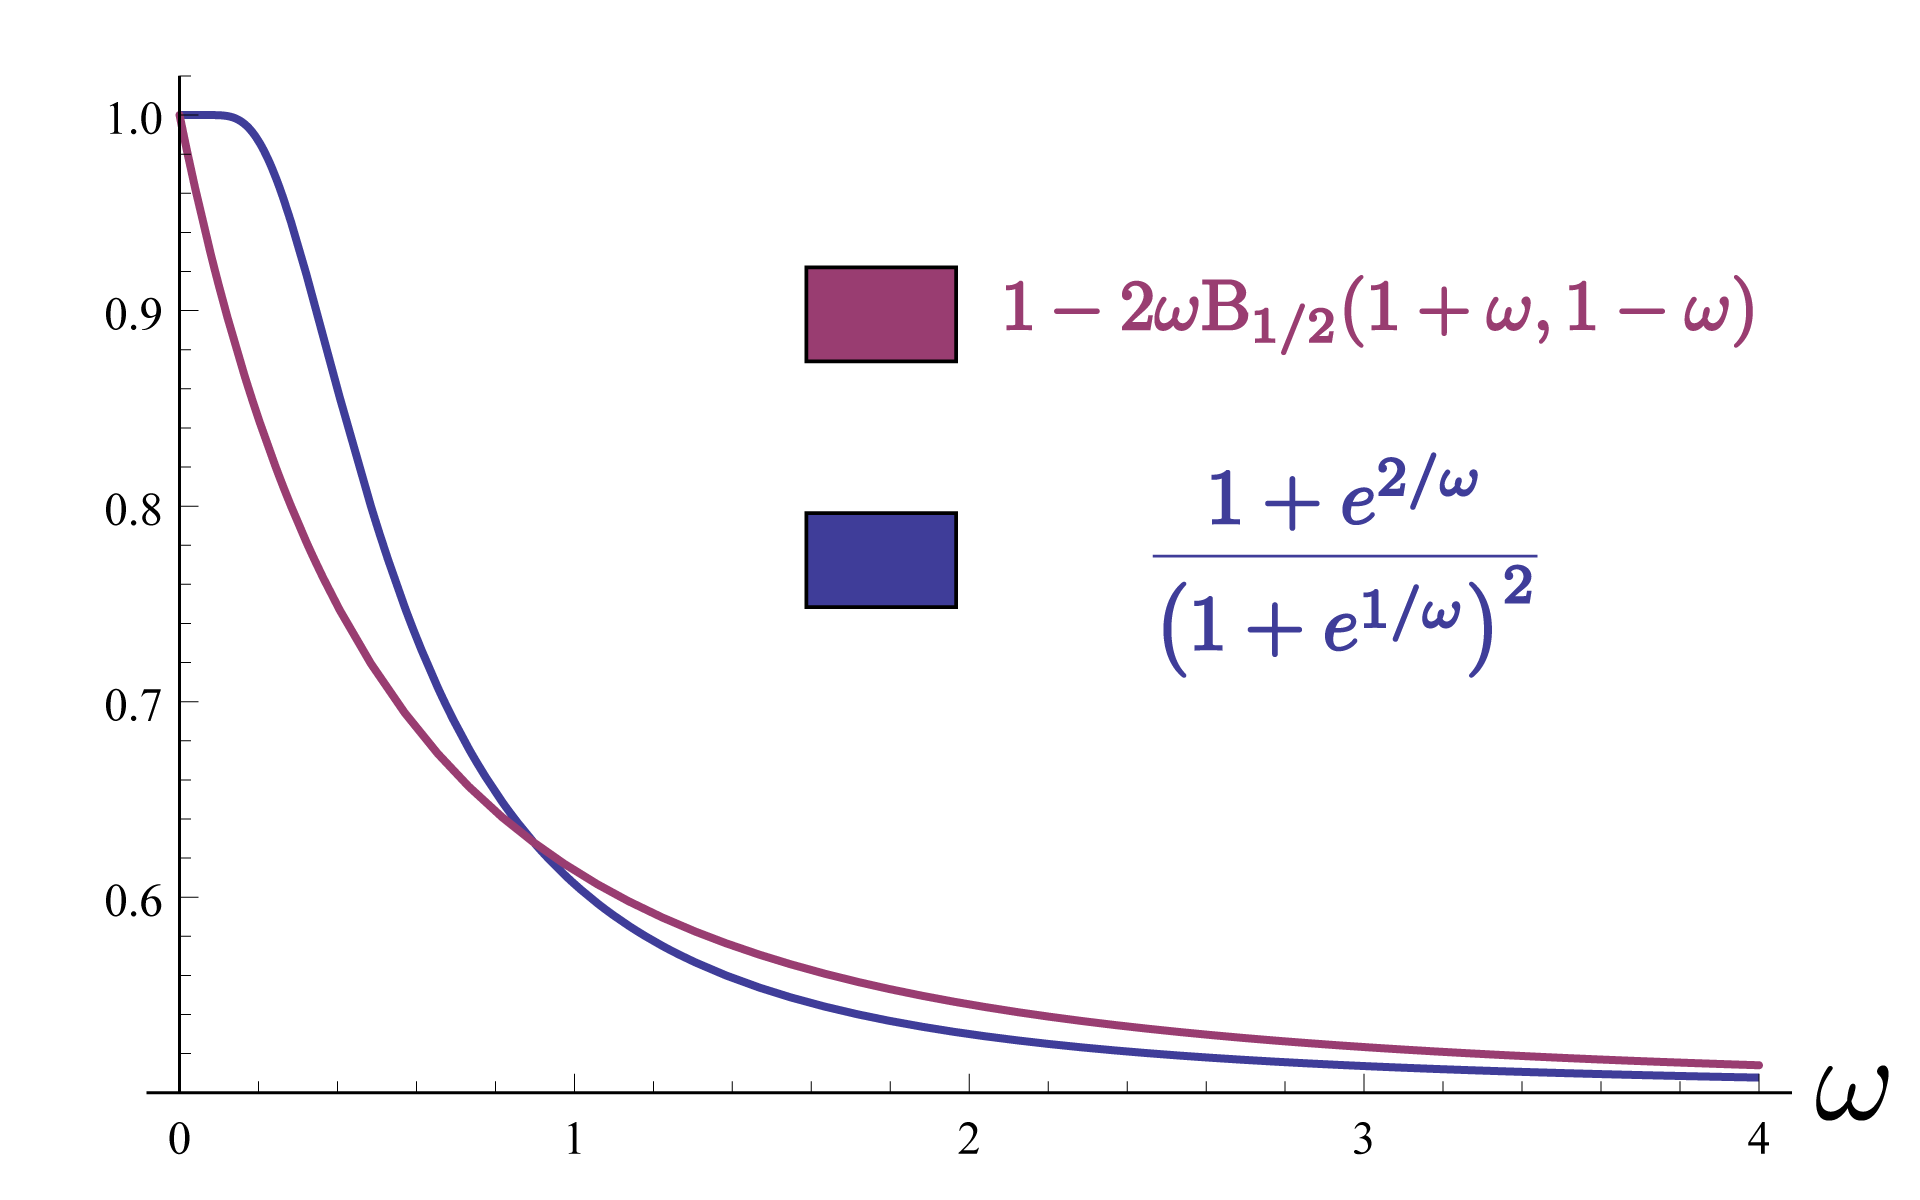
\includegraphics[width=13.0cm]{Figures/plot_psiofomega.png}\\
		\caption{ \textbf{The case $\nN =2$, evaluation of $\psi$ for different value of $\omega$}. 
		\label{plot_psiofomega} The purple solid line correspond to $\psi=1- 2 \omega \mathrm{B}_{1/2}(1+\omega,1-\omega)$, in this case the nematodes arrive at times exponentially distributed. The blue solid line correspond to $\psi=(1+q^2)/(1+q)^2$, in this case the nematodes arrive at constant times.
		}
	\end{figure}
 $\bullet$ If the birth rate of bacteria is far greater than the infection rate we have:
 \begin{equation}
 \tau \ll \lambda \Rightarrow q \gg 1 \Rightarrow R \simeq 1,
 \end{equation}
 The probability of identity is close to one, all bacteria are clones from the same lineage (same infecting nematode).
 $\bullet$ If the birth rate of bacteria is far lower than the infection rate we have:
 \begin{equation}
 \tau \gg \lambda \Rightarrow q \simeq 1 + \frac{\lambda }{\tau } \Rightarrow R \simeq 
  \dfrac{\dfrac{\lambda}{\tau}\left( \dfrac{\nN\lambda}{\tau} +2\right)}{\left( \dfrac{\lambda}{\tau} +2\right)\dfrac{\nN\lambda}{\tau}} \simeq \dfrac{1}{\nN}.
 \end{equation}
 The probability of identity is close to $1/ \nN$, as if all nematodes infected simultaneously the insect.
\section{Biological model and Relatedness.}
\label{section_life_cycle}
In this section, we seek to compute the relatedness in a biological model, at critical point of the life cycle of the bacteria.
 \paragraph{Notation} $ $\\
 $\bullet \quad t \in [0, t_{\mathrm{max}}]$, the time variable along the growth\\
 $\bullet \quad Q_0^{\mathrm{J}}$ the probability of identity of two bacteria in the same nematode during the free state\\
 $\bullet \quad Q_1^{\mathrm{J}}$ the probability of identity of two bacteria in different nematodes during the free state\\
 $\bullet \quad Q_0(t)$ the probability of identity of two bacteria in the same insect during growth\\
 $\bullet \quad Q_1(t)$ the probability of identity of two bacteria in different insects during growth\\
 $\bullet \quad Q_0'(t)$ is $Q_0(t)$ in the next cycle\\
 $\bullet \quad Q_1'(t)$ is $Q_1(t)$ in the next cycle\\
 $\bullet \quad \nI$ the number of insects\\
 $\bullet \quad \nN $ the number of nematodes infecting the insect\\
 $\bullet \quad \psi(t)={\mathbb E} \left[ \displaystyle  \sum_{i=1}^\nN  Z_i (t_{\mathrm{max}}) \right]$ the probability of identity of two bacteria in the same insect.
 
  \begin{figure}[H]
	  \centering
       \includegraphics[width=13.0cm]{Figures/life_cycle.png}\\
		\caption{ \textbf{The life cycle.}
		}
	\end{figure}
 The recursion equations describing the probabilities of identity are:
  \begin{subequations}
  \begin{numcases}{}
      		Q_0^{\mathrm{J}} = 1 \\
    		Q_1^{\mathrm{J}} = \dfrac{Q_0(t_{\mathrm{max}})}{\nI} +\dfrac{\nI-1}{\nI} Q_1(t_{\mathrm{max}})\\
    		Q_1'(t) = Q_1^{\mathrm{J}}\\
    		Q_0'(t) = {\mathbb E} \left[ \displaystyle  \sum_{i=1}^\nN  Z_i (t) \right] + Q_1^{\mathrm{J}} \left( 1 - {\mathbb E}\left[ \displaystyle  \sum_{i=1}^\nN Z_i(t) \right] \right).
  \end{numcases}
 \end{subequations}
 Hence, in a more compact way: 
  \begin{subequations}
  \begin{numcases}{}
      		Q_0'(t_{\mathrm{max}}) = \psi + \left( \dfrac{Q_0(t_{\mathrm{max}})}{\nI}+\dfrac{\nI-1}{\nI} Q_1(t_{\mathrm{max}}) \right) (1 -\psi) \\
    		    		Q_1'(t_{\mathrm{max}}) = \dfrac{Q_0(t_{\mathrm{max}})}{\nI}+\dfrac{\nI-1}{\nI} Q_1(t_{\mathrm{max}}),
  \end{numcases}
 \end{subequations}
  \subsection{Derivation of relatedness for low mutation rate.}
Taking mutation rate $u$ into account, in a similar fashion to \cite{rousset2004genetic}, the recursion equations become: 
  \begin{subequations}
  \begin{numcases}{}
      		Q_0'(t_{\mathrm{max}}) = (1-u)^2 \left[ \psi + \left( \dfrac{Q_0(t_{\mathrm{max}})}{\nI}+\dfrac{\nI-1}{\nI} Q_1(t_{\mathrm{max}}) \right) (1 -\psi) \right] \\
    		    		Q_1'(t_{\mathrm{max}}) = (1-u)^2 \left[ \dfrac{Q_0(t_{\mathrm{max}})}{\nI}+\dfrac{\nI-1}{\nI} Q_1(t_{\mathrm{max}}) \right].
  \end{numcases}
 \end{subequations}
 At equilibrium, $Q_0'(t_{\mathrm{max}})=Q_0(t_{\mathrm{max}})$ and $Q_1'(t_{\mathrm{max}})=Q_1(t_{\mathrm{max}})$ and the recursion equations are:
 \begin{subequations}
  \begin{numcases}{}
      		Q_0(t_{\mathrm{max}}) = (1-u)^2 \left[ \psi + \left( \dfrac{Q_0(t_{\mathrm{max}})}{\nI}+\dfrac{\nI-1}{\nI} Q_1(t_{\mathrm{max}}) \right) (1 -\psi) \right] \\
    		    		Q_1(t_{\mathrm{max}}) = (1-u)^2 \left[ \dfrac{Q_0(t_{\mathrm{max}})}{\nI}+\dfrac{\nI-1}{\nI} Q_1(t_{\mathrm{max}}) \right].
  \end{numcases}
 \end{subequations}
 Leading to the unique solution:
 \begin{align}
 Q_0(t_{\mathrm{max}}) &= \dfrac{ (1-u)^2 [u (2 - u)(\nI-1) +1 ]\psi }{ u (2-u )(\nI - \psi )+\psi }\\
 Q_1(t_{\mathrm{max}}) &= \dfrac{(1- u )^4 \psi}{u (2-u) (\nI - \psi ) +\psi}.
 \end{align}
 And the relatedness is: 
 \begin{equation}
 R(u)=\dfrac{Q_0(t_{\mathrm{max}})-Q_1(t_{\mathrm{max}})}{1-Q_1(t_{\mathrm{max}})}=\dfrac{(1-u)^2 \nI \psi}{\nI +(1-u)^2 \psi}.
 \end{equation}
And thus by taking the limit for low mutation rate ($u \rightarrow 0$), the relatedness becomes:
 \begin{equation}
 R \simeq \lim_{u \to 0} R(u)=\dfrac{\nI \psi}{\nI + \psi}=\dfrac{\psi}{1+ \dfrac{\psi}{\nI}}. \label{R=psi(nI)}
 \end{equation}
  \begin{align}
  R & \simeq \dfrac{\psi}{1+ \dfrac{\psi}{n_{I}}} \simeq \dfrac{(q-1)(q^\nN +1)}{(q+1)(q^\nN -1)} \left( 1+ \dfrac{(q-1)(q^\nN +1)}{\nI (q+1)(q^\nN -1)} \right)^{-1} \text{ by }\eqref{R=psi(nI)} \text{ and } \eqref{psi}\\
    &= \dfrac{(q-1)(q^\nN+1)}{ (q+1)(q^\nN -1)+ \dfrac{(q-1)(q^\nN +1)}{\nI}}.
 \end{align}
\subsection{Derivation of relatedness for infinite number of insects.}
Under the assumption of an infinite number of demes ($\nI \rightarrow \infty$), both $Q_1^{\mathrm{J}}$ and $Q_1(t)$ equal $0$ \cite{rousset2004genetic}. Thus the recursion equation at equilibrium for $Q_0(t_{\mathrm{max}})$ is solve unambiguously and give the relatedness $R$:
 \begin{equation}
 R \simeq \psi \simeq  \dfrac{(q-1)(q^\nN +1)}{(q+1)(q^\nN -1)}  \text{ by } \eqref{psi}
 \end{equation}
 It is worth noting that the relatedness does not depend on the number of bacteria initially brought by the nematode ($r$), nor on the the total population size when the bacteria stop growing exponentially. 
 This formula is valid only if the population of bacteria is growing exponentially at the time the last nematode infected the insect.
\section{Fitness function and derivation of equilibrium.}
 \label{section_fitness}
 In this section we make use of the previous results for the derivation of evolutionary stable strategies.
 \subsection{Nematodes feeding bacteria}
 \label{section_fitness_sub_feeding}
 In this case we are interested the nematodes feeding themselves of bacteria, after bacteria finished growing exponentially. We assume the bacteria can choose to sacrifice itself to nourish a nematode and thus increase the fitness of this focal nematode.
  \paragraph{Notation} $ $\\
 $\bullet \quad \nI$ the number of insects \\
 $\bullet \quad R$ the relatedness as previously \\
 $\bullet \quad z$ the phenotype of bacteria measuring the probability the individual(s) will sacrifice it(them)self to feed a nematode\\
 $\bullet \quad z_\bullet $ the phenotype $z$ for the focal individual\\
 $\bullet \quad z_j$ the phenotype $z$ for the individuals in the $j$th deme (the insect)\\
 $\bullet \quad \mathbf{z}=(z_1,\cdots,z_{\nI})$ the vector of $z_j$\\
 $\bullet \quad z_0^{\mathrm{R}}$ the average phenotype $z$ for the individuals in the same deme as the focal individual\\
 $\bullet \quad \bar{z}=\sum_k z_k / (\nI -1) $ the average phenotype $z$ for the individuals in demes different from the focal individual\\
 $\bullet \quad f (x)=ax+b$, $a>0$ a linear function describing the number of nematodes exiting the insect due to the phenotype (sacrifice) of bacteria.\\
 $\bullet \quad m=\sum_{i=1}^\nN r q^{i-1}$ the total number of bacteria released in the insect at the moment of the last infection by nematodes.
 
 
 
 We assume the following life cycle, focusing on one particular individual in the $j$th insect:
 
 
 $\bullet$ (1) Starting when the last nematode infected the insect, previous result showed that the relatedness is fixed and the exponential growth and final population size has a negligible impact on relatedness
 
 
 $\bullet$ (2) $J_{\mathrm{B}}$ bacteria are produced by the focal bacteria, they are in competition with $J_{\mathrm{B}} m$ bacteria in the same insect (including those of the focal individual).
 
 
 $\bullet$ (3) After the nematode eat from the bacteria, there is only $J_{\mathrm{B}}(1-z_\bullet)$ offspring of the focal individual competing with $J_{\mathrm{B}} m (1-z_j)$ offspring produced in the same insect (including those of the focal individual)
 
 
 $\bullet$ (4) $J_{\mathrm{N}} f(z_j)$ nematodes are produced from the $j$th insect, they are in competition with $\sum_{i=1}^{\nI} J_\mathrm{N} f(z_i)$ nematodes produced by all insect (including those produced by the insect of the focal individual)
 
 
 $\bullet$ (5) Only $\nN \nI$ nematodes will infect the next generation of insects. Since all nematodes are equivalent, the probability of being the $i$th $(1 \leq i \leq \nN)$ nematode infecting the insect 
is uniform, thus with probability $1/\nN$.If the nematode is the $i$th infecting the insect, the number of bacteria from this nematode at the moment of the last infection by nematodes is $r q^{i-1}$.
Thus, in expectation, there is $\nN \nI (\sum_{i=1}^\nN \nN^{-1}  r q^{i-1})=\nI m$ offspring of the focal one in the next cycle, conditioning on the carrying nematodes being from the one that succeeded their infection in the next cycle. 
Putting together all parts of the cycle, we can compute $ w_j(z_\bullet , \mathbf{z} )$, the fitness of a focal individual in deme $j$:
 \begin{align}
 w_j(z_\bullet , \mathbf{z} ) &= \dfrac{J_{\mathrm{B}}(1-z_\bullet)}{J_{\mathrm{B}} m (1- z_j)}\dfrac{ J_\mathrm{N} f(z_j)}{\sum_{i=1}^{\nI} J_\mathrm{N}  f(z_i)} \nI m \\
 &= \dfrac{1-z_\bullet}{1- z_j}\dfrac{\nI f(z_j)}{\sum_{i=1}^{\nI} f(z_i)} \\
  &= \dfrac{1-z_\bullet}{1- z_j}\dfrac{\nI (a z_j +b) }{\sum_{i=1}^{\nI} (a z_i +b)}.
 \end{align} 
 Since all demes are equivalent, for all demes $k$ different from the focal one, the $z_k$ variables contribute identically to the fitness measure. We write the fitness as a function of $z_\bullet$, $z_0^{\mathrm{R}}$ and $\bar{z}$:
  \begin{align}
 w(z_\bullet ,z_0^{\mathrm{R}} , \bar{z} ) &= \dfrac{1-z_\bullet}{1- z_0^{\mathrm{R}}}\dfrac{\nI (a z_0^{\mathrm{R}} +b) }{(a z_0^{\mathrm{R}} +b)+ b(\nI -1) +a \bar{z} (\nI-1)} \\
 &= \dfrac{1-z_\bullet}{1- z_0^{\mathrm{R}}}\dfrac{ a z_0^{\mathrm{R}} +b }{a \left( \dfrac{z_0^{\mathrm{R}}}{\nI} +\dfrac{\nI-1}{\nI} \bar{z} \right) +b}.
  \end{align}
  Under the model of infinite number of demes (insects), the fitness reduces to:
  \begin{equation}
  w(z_\bullet ,z_0^{\mathrm{R}} , \bar{z} ) \simeq \lim_{\nI \rightarrow \infty} w_j(z_\bullet ,z_0^{\mathrm{R}} , \bar{z} ) = \dfrac{1-z_\bullet}{1- z_0^{\mathrm{R}}}\dfrac{a z_0^{\mathrm{R}} +b }{a \bar{z} +b}.
  \end{equation}
  We then compute the partial derivative of the fitness with regard to $z_\bullet$ and $z_0^{\mathrm{R}}$ and evaluate them at $z$:
  \begin{equation}
  \dfrac{\partial w(z_\bullet ,z_0^{\mathrm{R}} , \bar{z} )}{\partial z_\bullet} = \dfrac{a z_0^{\mathrm{R}} +b }{ ( z_0^{\mathrm{R}} - 1) (a \bar{z} +b) } \Rightarrow \left. \dfrac{\partial w(z_\bullet ,z_0^{\mathrm{R}} , \bar{z} )}{\partial z_\bullet} \right\vert_{z_\bullet = z_0^{\mathrm{R}} = \bar{z}=z} = \dfrac{1}{ z-1 }.
  \end{equation}
  \begin{equation}
  \dfrac{\partial w(z_\bullet ,z_0^{\mathrm{R}} , \bar{z} )}{\partial z_0^{\mathrm{R}}} = \dfrac{(z_\bullet - 1)(a +b)}{(z_0^{\mathrm{R}} - 1)^2(a \bar{z} +b)} \Rightarrow \left. \dfrac{\partial w(z_\bullet ,z_0^{\mathrm{R}} , \bar{z} )}{\partial z_0^{\mathrm{R}}} \right\vert_{z_\bullet = z_0^{\mathrm{R}} = \bar{z}=z} = \dfrac{a +b}{( z - 1 )(a z +b)}.
  \end{equation}
  Solving $\left. \dfrac{\partial w}{\partial z_\bullet} \right\vert_{z^*} + \left. \dfrac{\partial w}{\partial z_0^{\mathrm{R}}} \right\vert_{z^*} R =0 $ yields a candidate evolutionary stable strategy, see \cite{rousset2004genetic}.
    \begin{equation}
  \dfrac{1}{ 1 - z^* } + \dfrac{a +b}{(1- z^*)(a z^* +b)}R =0
  \end{equation}
  \begin{equation}
  \iff
  \end{equation}
  \begin{equation}
  z^*=\dfrac{R(a+b)-b}{a}=R(1+c)-c \text{ where }c=\dfrac{b}{a}.
  \end{equation}
  In the special case $c=0$, the phenotype is the relatedness:
  \begin{equation}
  z^*=R.
  \end{equation} 
  It is worth noting that if $R<\dfrac{c}{c+1}$, then the candidate evolutionary stable strategy is no cooperation $(z^*=0)$.
  
  \subsection{Birth rate trade-off}
 In this case we are interested in a trade-off between birth rate and the number of nematodes escaping the insect. The ground for this assumption is that bacteria that do not dedicate themselves to growth can increase the fitness of the hosted nematodes using numerous strategies. For example they can produce bactericides or fungicides that kill-off unwanted guests, thus increasing the foraging of the host by the nematodes. 
  \paragraph{Notation} $ $\\
 $\bullet \quad \nI$ the number of insects \\
 $\bullet \quad \lambda$ the phenotype of bacteria measuring the birth rate\\
  $\bullet \quad R_{i}(\lambda)$ the relatedness as a function of lambda, when $i$ nematodes infected the insect \\
 $\bullet \quad \lambda_\bullet $ the phenotype $\lambda$ for the focal individual\\
 $\bullet \quad \lambda_j$ the phenotype $\lambda$ for the individuals in the $j$th deme (the insect)\\
 $\bullet \quad \mathbf{\lambda}=(\lambda_1,\cdots,\lambda_{\nI})$ the vector of $\lambda_j$\\
 $\bullet \quad \lambda_0^{\mathrm{R}}$ the average phenotype $\lambda$ for the individuals in the same deme as the focal individual\\
 $\bullet \quad \bar{\lambda}=\sum_k \lambda_k / (\nI -1) $ the average phenotype $\lambda$ for the individuals in demes different from the focal individual\\
 $\bullet \quad f (x)=ax+b$, $a<0$ a linear function describing the number of nematodes exiting the insect due to the phenotype of bacteria.
 
We assume the following life cycle, focusing on one particular individual in the $j$th insect:


 $ \bullet$ (1) In the first case, we assume the focal mutant bacterium belongs to the first nematode (with probability 1/2). The number of offspring from the focal bacteria is $e^{\lambda_\bullet \tau^{-1}}$ when the second nematode arrives. Once the exponential growth stops, the number of 
 bacteria from the focal one is thus $e^{\lambda_\bullet(\tau^{-1}+ t_\mathrm{x})}$. Moreover we have the relation $M=re^{\lambda_j(\tau^{-1}+ t_\mathrm{x})}+re^{\lambda_j t_\mathrm{x}} \iff t_\mathrm{x} = \mathrm{ln}(M/(re^{\lambda_j\tau^{-1}}+r))/ \lambda_j$, where $M$ is maximum number of bacteria the insect can carry. Thus the number of offspring from the focal individual is $e^{\lambda_\bullet\tau^{-1}} (M/(re^{\lambda_j\tau^{-1}}+r))^{\lambda_\bullet / \lambda_j}$
 
 $ \bullet$ (2) If the focal bacteria belongs to the second arriving nematode (with probability 1/2), then the number of offspring is $ (M/(re^{\lambda_j\tau^{-1}}+r))^{\lambda_\bullet / \lambda_j}$
 
 
 $\bullet$ (3) The offspring of the focal bacteria are competing with a total of $M$ offspring.
 
 
 $\bullet$ (4) $J_{\mathrm{N}} f(\lambda_j)$ nematodes are produced from the $j$th insect, they are in competition with $\sum_{i=1}^{\nI} J_\mathrm{N} f(z_i)$ nematodes produced by all insect (including those produced by the insect of the focal individual)
 
 
 $\bullet$ (5) Only $2 \nI$ nematodes will infect the next generation of insects, producing $r$ descending offspring each.
 Putting together all the part, we have: 
 \begin{align}
 w_j(\lambda_\bullet , \mathbf{\lambda} ) &= \dfrac{e^{\lambda_\bullet\tau^{-1}}+1}{2} \left( \dfrac{M}{re^{\lambda_j\tau^{-1}}+r} \right)^{\dfrac{\lambda_\bullet }{\lambda_j}} \dfrac{1}{M}\dfrac{  f ( \lambda_j )}{\sum_{i=1}^\nI f ( \lambda_i )} 2\nI r  \\
 \end{align} 
% Since all demes are equivalent, for all demes $k$ different from the focal one, the $z_k$ variables contribute identically to the fitness measure. We write the fitness as a function of $z_\bullet$, $z_0^{\mathrm{R}}$ and $\bar{z}$:
%  \begin{align}
% w(\lambda_\bullet ,\lambda_0^{\mathrm{R}} , \bar{\lambda} ) &=  \dfrac{e^{\lambda_\bullet-\lambda_0^{\mathrm{R}}} \nI (a \lambda_0^{\mathrm{R}} +b) }{(a \lambda_0^{\mathrm{R}} +b)+ b(\nI -1) +a \bar{\lambda} (\nI-1)} \\
% &=  \dfrac{e^{\lambda_\bullet-\lambda_0^{\mathrm{R}}} ( a \lambda_0^{\mathrm{R}} +b ) }{a \left( \dfrac{\lambda_0^{\mathrm{R}}}{\nI} +\dfrac{\nI-1}{\nI} \bar{\lambda} \right) +b}.
%  \end{align}
%  Under the model of infinite number of demes (insects), the fitness reduces to:
%  \begin{equation}
%  w(\lambda_\bullet ,\lambda_0^{\mathrm{R}} , \bar{\lambda} ) \simeq \lim_{\nI \rightarrow \infty} w_j(\lambda_\bullet ,\lambda_0^{\mathrm{R}} , \bar{\lambda} ) = \dfrac{e^{\lambda_\bullet-\lambda_0^{\mathrm{R}}} (a \lambda_0^{\mathrm{R}} +b )}{a \bar{\lambda} +b}.
%  \end{equation}
%  We then compute the partial derivative of the fitness with regard to $z_\bullet$ and $z_0^{\mathrm{R}}$ and evaluate them at $z$:
%  \begin{equation}
%  \dfrac{\partial w(\lambda_\bullet ,\lambda_0^{\mathrm{R}} , \bar{\lambda} )}{\partial \lambda_\bullet} = w(\lambda_\bullet ,\lambda_0^{\mathrm{R}} , \bar{\lambda} ) \Rightarrow \left. \dfrac{\partial w(\lambda_\bullet ,\lambda_0^{\mathrm{R}} , \bar{\lambda} )}{\partial \lambda_\bullet} \right\vert_{\lambda} = 1.
%  \end{equation}
%  \begin{equation}
%  \dfrac{\partial w(\lambda_\bullet ,\lambda_0^{\mathrm{R}} , \bar{\lambda} )}{\partial \lambda_0^{\mathrm{R}}} =\dfrac{ e^{\lambda_\bullet-\lambda_0^{\mathrm{R}}} (a (1+ \lambda_0^{\mathrm{R}}) -b) }{a \bar{\lambda} +b} \Rightarrow \left. \dfrac{\partial w(\lambda_\bullet ,\lambda_0^{\mathrm{R}} , \bar{\lambda} )}{\partial \lambda_\bullet} \right\vert_{\lambda} = \dfrac{a}{a \lambda +b}-1.
%  \end{equation}
%  Solving $\left. \dfrac{\partial w}{\partial \lambda_\bullet} \right\vert_{\lambda^*} + \displaystyle \sum_{i=1}^\nN  R_i ( \lambda^*) \left. \dfrac{\partial w}{\partial \lambda_0^{\mathrm{R}}} \right\vert_{\lambda^*} =0 $ yields a candidate evolutionary stable strategy, see \cite{rousset2004genetic}.
%\begin{align}
%1=\sum_{i=1}^\nN  \dfrac{(e^{  \lambda^* / \tau}-1)((e^{\lambda^* / \tau})^i +1)}{(e^{\lambda^* / \tau}+1)((e^{\lambda^* / \tau})^i -1)} (1-\dfrac{a}{a \lambda^* +b}) \text{ by } \eqref{R=psi(nI)}
%\end{align}
\section{Supplementary materials}
\subsection{Exponential growth of bacteria, birth-death process.}
In this section we extend the pure birth process to a birth-death process, adding linear a death process.
 \paragraph{Notation} $ $\\
 $\bullet \quad t \in \mathbb{R}_+$, the time variable along the growth\\
 $\bullet \quad \pr_n(t)$, the probability that the population at time $t$ is of size $n$.\\
 $\bullet \quad N(t)$, the random variable with law $\pr(N(t)=n)=\pr_n(t)$\\
 $\bullet \quad r$ the initial population size\\
 $\bullet \quad \lambda$ the infinitesimal birth rate\\
 $\bullet \quad \mu$ the infinitesimal death rate\\
 
 
 The process is such that each bacteria has an independent birth rate $\lambda$ and a death rate $\mu$. Thus the forward equation is:   
 \begin{subequations}
  \begin{numcases}{}
    \sum_{i \geq 1} \pr_n(t)=1\\
    \pr_{r}(0)=1 \\
    \pr'_i(t)=\lambda (i-1) \pr_{i-1}(t)+\mu (i+1)\pr_{i+1}(t)-i(\lambda+\mu)\pr_i(t)\text{ for } i\geq 1 \label{eq:dif:BD}
  \end{numcases}
 \end{subequations}
Multiply the differential equation \eqref{eq:dif:BD} by $(s^1,s^2,s^3,\hdots)$ and add. We obtain a single partial differential equation:
 \begin{subequations}
  \begin{numcases}{}
    		G(s,0)=s^{r} \\
    		G(1,t)=1 \\
    		G(0,t)=0 \\
    		\dfrac{\partial G(s,t)}{\partial t} = (\lambda s -\mu)(s-1) \dfrac{\partial G(s,t)}{\partial s} \text{ for } s \in [0,1] \label{eq:dif:BD:partial}
 \end{numcases}
 \end{subequations}
 with $\displaystyle G(s,t)=\sum_{i=1}^{\infty} \pr_i(t)s^i=\mathbb{E}[ s^{N(t)}] $ the probability generating function of $N(t)$. \\
The probability generating function satisfying this equation is :
\begin{equation}
\displaystyle  G(s,t)=  \left( \dfrac{\mu (1-s)-(\mu- \lambda s) \exp^{-(\lambda - \mu )t}}{\lambda (1-s)-(\mu -\lambda s) \exp^{-(\lambda -\mu )t}} \right)^{r} \text{ for } s \in [0,1].
\end{equation}
$N(t)=0$ is an absorbing state, thus the behavior of this Markov chain is more complicated and calculus of Identity by descendant is intractable. 
\subsection{Logistic growth of bacteria}
In this section we extend the pure death processes to a birth-death process, adding non linear a death process due to competition.
 \paragraph{Notation} $ $\\
 $\bullet \quad t \in \mathbb{R}_+$, the time variable along the growth\\
 $\bullet \quad \pr_n(t)$, the probability that the population at time $t$ is of size $n$.\\
 $\bullet \quad N(t)$, the random variable with law $\pr(N(t)=n)=\pr_n(t)$\\
 $\bullet \quad r$ the initial population size\\
 $\bullet \quad \lambda$ the infinitesimal birth rate\\
 $\bullet \quad c$ the infinitesimal competition rate\\ 
 
 
 
 The process is such that each bacteria has an independent birth rate $\lambda$, and the death is only due to competition such that each bacteria dies out a rate $n\lambda$, where $n$ is the number of other bacteria. Thus the forward equation is:   
 \begin{subequations}
  \begin{numcases}{}
    \sum_{i \geq 1} \pr_n(t)=1\\
    \pr_{r}(0)=1 \\
    \pr'_i(t)=(i-1)\lambda \pr_{i-1}(t)+ci(i+1)\pr_{i+1}(t)-i(\lambda+c(i-1))\pr_i(t)\text{ for } i\geq 1 \label{eq:dif}
  \end{numcases}
 \end{subequations}
Multiply the differential equation \eqref{eq:dif} by $(s^1,s^2,s^3,\hdots)$ and add. We obtain a single partial differential equation:
 \begin{subequations}
  \begin{numcases}{}
    		G(s,0)=s^{r} \\
    		G(1,t)=1 \\
    		G(0,t)=0 \\
    		\dfrac{\partial G(s,t)}{\partial t} = \lambda s(s-1) \dfrac{\partial G(s,t)}{\partial s} + c s(1-s) \dfrac{\partial^2 G(s,t)}{\partial s^2} \text{ for } s \in [0,1] \label{eq:dif:partial}
 \end{numcases}
 \end{subequations}
 with $\displaystyle G(s,t)=\sum_{i=1}^{\infty} \pr_i(t)s^i=\mathbb{E}[ s^{N(t)}] $ the probability generating function of $N(t)$. \\
At equilibrium, with $\omega = \lambda / c $, the probability generating function satisfying this equation is :
\begin{equation}
\displaystyle  G(s,\infty)= \sum_{i\geq 1} \dfrac{e^{-\omega}}{1-e^{-\omega}} \dfrac{ \omega^i}{i!} s^i = \dfrac{e^{-\omega}}{1-e^{-\omega}} \left( e^{s \omega} -1 \right) \text{ for } s \in [0,1]
\end{equation}
  And the associated limiting distribution is that of a Poisson variable, conditioned on being positive: 
 \begin{equation}
 \displaystyle \pr_i(\infty)=\dfrac{e^{-\omega}}{1-e^{-\omega}} \dfrac{ \omega^i}{i!} \text{ for } i\geq 1
 \end{equation}
 Denote $G(s,t)=e^{s \lambda / (2c) }K(s,t)$ and the \eqref{eq:dif:partial} become :
 \begin{subequations}
  \begin{numcases}{}
    		K(0,t)=0 \\
    		\dfrac{\partial K(s,t)}{\partial t} = \dfrac{\lambda^2}{2c} s(s-1) K(s,t) + c s(1-s) \dfrac{\partial^2 K(s,t)}{\partial s^2} \text{ for } s \in [0,1] 
 \end{numcases}
 \end{subequations}
 Multiply the differential equation \eqref{eq:dif} by $(e^{-\theta},e^{-2\theta},e^{-3\theta},\hdots)$ and add. We obtain a single partial differential equation:
  \begin{subequations}
  \begin{numcases}{}
    		H(0,t)=1 \\
    		H(\theta ,0)=e^{-\theta r } \\
    		\dfrac{\partial H(\theta,t)}{\partial t} = \lambda (1-e^{-\theta}) \dfrac{\partial H(\theta,t)}{\partial \theta} + c (e^{\theta}-1) \left( \dfrac{\partial H(\theta,t)}{\partial \theta}+\dfrac{\partial^2 H(\theta,t)}{\partial \theta ^2} \right) \text{ for } \theta \in \mathbb{R_+}
 \end{numcases}
 \end{subequations}
 with $\displaystyle H(s,t)=\sum_{i=1}^{\infty} \pr_i(t)e^{-i \theta }=\mathbb{E}[ e^{-\theta N(t)}]$ the moment generating function of $N(t)$. \\
 \subsection{Probability of identity using probability generating functions.}
 \label{subsection_pgf}
 Following the notations of section \ref{section_PI}, we derived the probability of identity directly as function of the joint pgf of $N_i(t)$ and $N_+(t)$.
 Let $G_{N_i(t) ,N_+(t)}(s_i,s_+)$ be the pgf of the joint distribution of $N_i(t)$ and $N_+(t)$. We have the following relation:
 \begin{align}
 \displaystyle \int_0^1 \int_0^y \dfrac{\partial^2 }{\partial s_i^2} & \left( \dfrac{G_{N_i(t) ,N_+(t)}(s_i,s_+)}{s_+^2} \right)_{s_i =1} \ud s_+ \ud y \\
 &= \int_0^1 \int_0^y \dfrac{\partial^2 }{\partial s_i^2} \left( \sum_{n_i,n_+ \geq 1} \pr(N_i(t)=n_i \cap N_+(t)=n_+) s_+^{n_+ -2} s_1^{n_1} \right)_{s_i =1} \ud s_+ \ud y \\ 
 &= \sum_{n_i,n_+ \geq 1} \pr(N_i(t)=n_i \cap N_+(t)=n_+) \left.  \dfrac{\partial^2 s_i^{n_i}}{\partial s_i^2} \right\vert_{s_i=1} \int_0^1 \int_0^y s_+^{n_+-2} \ud s_+ \ud y\\
 &= \sum_{n_i  ,n_+ \geq 1} \pr(N_i(t)=n_i \cap N_+(t)=n_+) \dfrac{n_i(n_i-1)}{n_+(n_+-1)}\\
 &= \mathbb{E}\left[ Z_i(t) \right].
 \end{align}
 Moreover $G_{N_i(t) ,N_+(t)}(s_i,s_+)$ can be reduced to the product of two pgf: 
  \begin{align}
G_{N_i(t) ,N_+(t)}(s_i,s_+,t) &= \mathbb{E} [ s_i^{N_i(t)} s_+^{N_+(t)}] \\
		&= \mathbb{E} [ s_i^{N_i(t)} s_+^{N_i(t)+N_{-i}(t)}]\\
		&= \mathbb{E} [ (s_i s_+)^{N_i(t)} s_+^{N_{-i}(t)}] \\
		&= \mathbb{E} [ (s_i s_+)^{N_i(t)} ]\mathbb{E} [ s_+^{N_{-i}(t)}] \\
		&= G_{N_i(t)}(s_i s_+) G_{N_{-i}(t)}(s_+).
 \end{align}
 Hence, we have 
   \begin{align}
\displaystyle \int_0^1 \int_0^y \dfrac{\partial^2 }{\partial s_i^2} \left( \dfrac{G_{N_i(t) ,N_+(t)}(s_i,s_+)}{s_+^2} \right)_{s_i =1} \ud s_+ \ud y
 &= \int_0^1 \int_0^y \dfrac{\partial^2 }{\partial s_i^2} \left( \dfrac{ G_{N_i(t)}(s_i s_+) G_{N_{-i}(t)}(s_+)}{s_+^2} \right)_{s_i =1} \ud s_+ \ud y \\
  &= \int_0^1 \int_0^y \dfrac{G_{N_{-i}(t)}(s_+)}{s_+^2} \left. \dfrac{\partial^2  G_{N_i(t)}(s_i s_+)  }{\partial s_i^2} \right\vert_{s_i =1} \ud s_+ \ud y \\
    &= \int_0^1 \int_0^y G_{N_{-i}(t)}(s_+) \dfrac{\partial^2  G_{N_i(t)}(s_+)  }{\partial s_+^2} \ud s_+ \ud y.
 \end{align}
 Thus the PI is a function solely of $G_{N_{i}(t)}$ and $G_{N_{-i}(t)}$:
 \begin{equation}
 \displaystyle \mathbb{E}\left[ Z_i(t) \right]= \int_0^1 \int_0^y G_{N_{-i}(t)}(s) \dfrac{\partial^2 G_{N_i(t)}(s)}{\partial s^2} \ud s \ud y.
 \end{equation}
This can be evaluated with Mathematica and it gives the same result as previously.
\bibliographystyle{plain}
\bibliography{references,references_none_mendeley}
\end{document}


